\documentclass[a4paper]{article}
\usepackage[14pt]{extsizes} % для того чтобы задать нестандартный 14-ый размер шрифта
\usepackage[utf8]{inputenc}
\usepackage[english,main=russian]{babel}
\usepackage{setspace,amsmath}
\usepackage{subcaption}
\usepackage[final]{graphicx}
\usepackage{epstopdf}
\usepackage{mathtext}
\DeclareGraphicsExtensions{.pdf,.png,.jpg}
\usepackage[left=20mm, top=15mm, right=15mm, bottom=15mm, nohead, footskip=10mm]{geometry} % настройки полей документа
\usepackage{ragged2e}
\justifying

% =======================================================
% Далее титульный лист
% =======================================================

\begin{document}
\begin {center}
    \hfill \break
    \textbf{Федеральное государственное бюджетное образовательное учреждение высшего образования}\\
    \small{\textbf{«РЫБИНСКИЙ ГОСУДАРСТВЕННЫЙ АВИАЦИОННЫЙ ТЕХНИЧЕСКИЙ УНИВЕРСИТЕТ имени П. А. СОЛОВЬЁВА»}}\\
    \hfill \break
    \normalsize{Институт информационных технологий и систем управления}\\
    \hfill \break
    \normalsize{Кафедра математического и программного обеспечения электронных вычислительных средств}\\
    \hfill\break
    \hfill \break
    \hfill \break
    \hfill \break
    \large{Лабораторная работа №2}\\
    \normalsize{\textbf{Обработка данных в датасете "Абитуриенты"}}\\
    \hfill \break
    \hfill \break
    \hfill \break
    \normalsize{по дисциплине\\
Методы и алгоритмы анализа данных\\}
    \hfill \break
    \hfill \break
    \hfill \break
    \hfill \break
    \hfill \break
\end {center}

\begin {flushleft}
\normalsize{ 
    Выполнили студенты 
    группы ИВМ-22  
    \hfill Перхуров В. А. \\
    \hfill Беляев А. Е. \\
    \hfill \break
    Проверил: 
    \hfill Кулиманов И. Е. 
}
\end {flushleft}

\hfill \break
\hfill \break
\hfill \break
\hfill \break
\hfill \break
\hfill \break
\hfill \break

\begin{center} 
    Рыбинск 2022 
\end{center}
\thispagestyle{empty} 

% =======================================================
% Далее лист с заданием
% =======================================================

\newpage
\begin{center}
    \hfill \break
    \textbf{Задание}\\
\end{center}  
\normalsize{
    \textbf{Постановка задачи:}\\\\
    Цели:\\\\
    Провести анализ и обработку данных из заданного датасета "Абитуриенты"\\\\
    Задачи:\\
    \begin{enumerate}
        \item Какая причина выбора школы была самой частой? В качестве ответа приведите соответствующее значение признака.
        \item Найдите количество студентов, у родителей которых нет никакого образования.
        \item Найдите минимальный возраст учащегося школы Mousinho da Silveira.
        \item Найдите количество студентов, имеющих нечетное число пропусков.
        \item Найдите разность между средними итоговыми оценками студентов, состоящих и не состоящих в романтических отношениях. В качестве ответа приведите число, округленное до двух значащих цифр после запятой.
        \item Сколько занятий пропустило большинство студентов с самым частым значением наличия внеклассных активностей?
        \begin{itemize}
            \item Определить самое частое значение наличия внеклассных активностей (да или нет).
            \item Для группы студентов, соответствующей этому значению, рассмотреть значения признака «число пропусков».
            \item Для каждого значения числа пропусков посчитать, сколько студентов ему соответствует.
            \item Выбрать значение числа пропусков с наибольшим числом студентов.
        \end{itemize}
    \end{enumerate}
}

% =======================================================
% Далее листы с описанием датасетов
% =======================================================

\newpage
\begin{center}
    \hfill \break
    \section{Описание датасета "Абитуриенты"}
\end{center}
\normalsize{
    Набор данных представлен в CSV-файле. Каждая строчка наборов данных содержит следующие поля:
    \begin{enumerate} 
        \item school - тип школы ("GP" - Gabriel Pereira или "MS" - Mousinho da Silveira)
        \item sex - пол ("F" - female или "M" - male)
        \item age - возраст (от 15 до 22)
        \item address - откуда студент ("U" - urban или "R" - rural)
        \item famsize - размер семьи ("LE3" - меньше или равно 3 или "GT3" - больше 3)
        \item Pstatus - в каких отношениях родители ("T" - живут вместе "A" - раздельно)
        \item Medu - образование матери (0 - никакого, 1 - начальное образование (4 класса), 2 – от 5 до 9 классов, 3 –среднеспециальное или 4 – высшее)
        \item Fedu - образование отца (0 - никакого, 1 - начальное образование (4 класса), 2 – от 5 до 9 классов, 3 – среднеспециальное или 4 – высшее)
        \item Mjob - работа матери ("teacher", "health" care related, civil "services" (e.g. administrative or police), "at\_home" or "other")
        \item Fjob - работа отца ("teacher", "health" care related, civil "services" (e.g. administrative or police), "at\_home" or "other")
        \item reason - причина выбора школы (близко к дому — "home", репутация школы — "reputation", предпочтение некоторым предметам - "course" или "other")
        \item guardian - опекун ("mother", "father" или "other")
        \item traveltime - время от дома до школы (1 - меньше 15 мин., 2 - 15 до 30 мин., 3 - 30 мин. до 1 часа, или 4 - больше 1 часа)
        \item studytime - количество часов обучения в неделю (1 - меньше 2 часов, 2 - от 2 до 5 часов, 3 - от 5 до 10 часов, или 4 - больше 10 часов)
        \item failures - количество ранее не сданных предметов (n if 1 <= n < 3, else 4)
        \item schoolsup - дополнительные занятия (yes or no)
        \item famsup - помощь от семьи при выполнении заданий (yes or no)
        \item paid - дополнительные платные занятия (yes or no)
        \item activities - внеклассная деятельность (yes or no)
        \item nursery - посещал детский сад (yes or no)
        \item higher - желание высшего образования (yes or no)
        \item internet - домашний интернет (yes or no)
        \item romantic - состоит в романтических отношениях (yes or no)
        \item famrel - насколько хороши отношения в семье (от 1 - очень плохие до 5 - превосходные)
        \item freetime - наличие свободного времени после школы (от 1 - очень мало до 5 - очень много)
        \item goout - гуляет с друзьями (от 1 - редко до 5 - очень часто)
        \item Dalc - употребление алкоголя в будние дни (от 1 - очень редко до 5 - очень часто)
        \item Walc - употребление алкоголя в выходные (от 1 - очень редко до 5 - очень часто)
        \item health - текущее состояние здоровья (от 1 - очень плохое до 5 - очень хорошее)
        \item absences - количество школьных пропусков (от 0 до 93)
        \item G1 - оценка за первый семестр (от 0 до 20)
        \item G2 - оценка за второй семестр (от 0 до 20)
        \item G3 - итоговая оценка (от 0 до 20)
    \end{enumerate}
}

% =======================================================
% Далее листы с описанием выполнения работы
% =======================================================

\newpage
\begin{center}
\hfill \break
\section{Описание выполнения работы}
\end{center}

\subsection{Реализация программы для анализа датасета "Абитуриенты"}
\subsubsection{Используемые библиотеки}
\normalsize{
    При решении данной задачи была использована библиотека pandas (анализ данных).
}
\subsubsection{Ход работы и результат выполнения программы}
\normalsize{
    В ходе выполнения работы была написана программа, которя выводит результат анализа датасета в лог. На рисунке 1 показан данный вывод.
    
    \begin{figure}[h]
        \centering
        \graphicspath{{./}}
        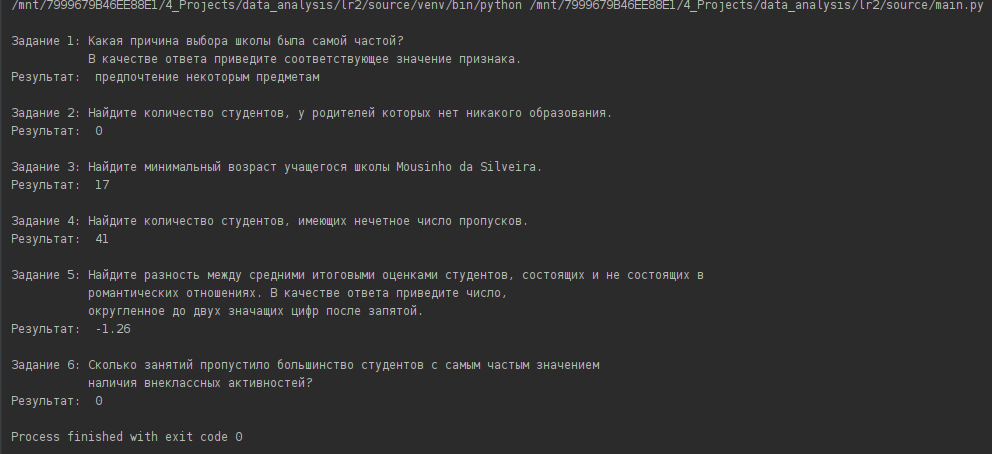
\includegraphics[scale=0.65]{programm_result.png}
        \caption{Результат работы программы}
    \end{figure} 
}
\subsubsection{Исходный текст программы}
\normalsize{
    \begin{verbatim}
import pandas as pd  # анализ данных

# Найти наиболее распространённое значение в датасете.
# Принимает набор данных и название столбца для определения 
# его самого частого значения.
def FindMostCommonValues(data, column_name):
    return pd.value_counts(data[column_name].values, sort=True).axes[0][0]


# Задание 1:
#           Какая причина выбора школы была самой частой?
#           В качестве ответа приведите соответствующее значение признака.
def FindMostCommonReasonForChoosingSchool(main_df):
    reason_values = {
        "home": "близко к дому",
        "reputation": "репутация школы",
        "course": "предпочтение некоторым предметам",
        "other": "предпочтение некоторым предметам",
    }

    # определение самой частой причины выбора школы
    reason = FindMostCommonValues(main_df, 'reason')

    print("""
Задание 1: Какая причина выбора школы была самой частой?
           В качестве ответа приведите соответствующее значение признака.
Результат: """, reason_values[reason])


# Задание 2:
#           Найдите количество студентов, у родителей которых 
#           нет никакого образования.
def FindNumberOfStudentsWhoseParentsHaveNoEducation(main_df):
    no_education_value = 0
    data = main_df[(main_df['Medu'] == no_education_value) &
                   (main_df['Fedu'] == no_education_value)]

    print("""
Задание 2: Найдите количество студентов, у родителей которых
           нет никакого образования.
Результат: """, len(data))


# Задание 3:
#           Найдите минимальный возраст учащегося школы 
#           Mousinho da Silveira.
def FindMinimumAgeOfStudentAtMousinhoDaSilveiraSchool(main_df):
    school_name = 'MS'
    data = main_df[(main_df['school'] == school_name)]

    print("""
Задание 3: Найдите минимальный возраст учащегося школы 
           Mousinho da Silveira.
Результат: """, min(data['age']))


# Задание 4:
#           Найдите количество студентов, 
#           имеющих нечетное число пропусков.
def FindNumberOfStudentsWhoHaveAnOddNumberOfAbsences(main_df):
    data = main_df[main_df['absences'] % 2 != 0]

    print("""
Задание 4: Найдите количество студентов, имеющих нечетное число пропусков.
Результат: """, len(data))


# Задание 5:
#           Найдите разность между средними итоговыми оценками студентов,
#           состоящих и не состоящих в романтических отношениях. 
#           В качестве ответа приведите число,
#           округленное до двух значащих цифр после запятой.
def FindDifferenceBetweenAverageFinalGradesOfStudentsInAndOutOfRomanticRelationships(main_df):
    data = main_df.groupby('romantic').describe()
    # "{:.2f}".format - округление до 2-х символов после запятой
    result_difference = "{:.2f}".format(data['G3', 'mean']['yes'] -
                                       data['G3', 'mean']['no'])

    print("""
Задание 5: Найдите разность между средними итоговыми оценками студентов,
           состоящих и не состоящих в романтических отношениях.
           В качестве ответа приведите число, 
           округленное до двух значащих цифр после запятой.
Результат: """, result_difference)


# Задание 6:
#           Сколько занятий пропустило большинство студентов 
#           с самым частым значением наличия внеклассных активностей?
def HowManyClassesDidMostStudentsWithMostFrequentValueOfHavingExtracurricularActivitiesMiss(main_df):
    activities_is_exist = FindMostCommonValues(main_df, 'activities')
    data_with_activities = main_df[main_df['activities'] ==
                           activities_is_exist]
    number_of_students_by_absences =     
        pd.value_counts(data_with_activities['absences'].values, 
                        sort=True)

    print("""
Задание 6: Сколько занятий пропустило большинство студентов
           с самым частым значением наличия внеклассных активностей?
Результат: """, number_of_students_by_absences.axes[0][0])


# Основная функция
def main():
    # 0 - Читаем датасет
    df = pd.read_csv('./math_students.csv', 
                     escapechar='`',
                     low_memory=False)
    # Задание 1
    FindMostCommonReasonForChoosingSchool(df)
    # Задание 2
    FindNumberOfStudentsWhoseParentsHaveNoEducation(df)
    # Задание 3
    FindMinimumAgeOfStudentAtMousinhoDaSilveiraSchool(df)
    # Задание 4
    FindNumberOfStudentsWhoHaveAnOddNumberOfAbsences(df)
    # Задание 5
    FindDifferenceBetweenAverageFinalGradesOfStudentsInAndOutOfRomanticRelationships(df)
    # Задание 6
    HowManyClassesDidMostStudentsWithMostFrequentValueOfHavingExtracurricularActivitiesMiss(df)


# Запускаем программу
main()
    \end{verbatim}
}
 
% =======================================================
% Далее лист с выводом о проделанной работе
% =======================================================

\newpage
\begin{center}
\hfill \break
\section{Вывод.}
\end{center} 
\normalsize{
    В результате выполнения лабораторной работы были проведёны анализ и обработка данных из заданного датасета "Абитуриенты".
    
    В ходе выполнения работы была написана программа, которая выполняют чтение датасета из фала в формате ".csv" и реализуют заданный функционал:
    \begin{enumerate}
        \item Найти самую частую причину выбора школы.
        \item Найти количество студентов, у которых родители не имеют никакого образования.
        \item Найти минимальный возраст учащегося школы Mousinho da Silveira.
        \item Найти количество студентов, имеющих нечетное число пропусков.
        \item Найти разность между средними итоговыми оценками студентов, состоящих и не состоящих в романтических отношениях.
        \item Найти количество занятий, пропущенных большинством студентов, у которых есть (или нет) внеклассная активность (в зависимости от того, что чаще встречается).
    \end{enumerate}
}
\end{document}